\section{Simulaciones y experimentos}
    En esta sección se realizarán simulaciones y comparaciones entre distintos sistemas. Para demostrar la idea básica de sistema TIIR, se comenzerá examinando el sistema tal que

    \begin{equation}
      H(z) = \frac{z^{2}}{z^{2} - 1.9 \: z + 0.98} = \frac{B^{+}(z)}{A^{+}(z)}
    \end{equation}

    el cual se deseará truncar luego de un $N = 300 \: [\text{muestras}]$ arbitrario; esto es, se desea obtener una respuesta FIR de 301 pasos. Se comienza entonces formando el polinio de cancelación de cola como en la Eq. \ref{eq:25}, realizando división sintética de $z^{N} \: B(z)$  por $A(z)$, lo que resulta en el resto

    \begin{equation}
      B^{\prime +}(z) = - 0.162126 \: z + 0.13977
    \end{equation}

    De esta manera, se puede definir $H_{FIR}^{+}(z)$ según la Ec. \ref{eq:42}

    \begin{align}
      H_{FIR}^{+}(z) =& \frac{B(z) - z^{-N} \: B^{\prime + }(z)}{A(z)} \nonumber \\
      =& \frac{z^{2} + z^{-N} \: \left( - 0.162126 \: z + 0.139977 \right)}{z^{2} - 1.9 \: z + 0.98}
    \end{align}

    Entonces, se definen los coeficientes de $H_{FIR}^{+}(z)$  como

    \begin{itemize}
      \item $a = 0.162126$
      \item $b = 0.139977$
      \item $p = 1.9$
      \item $q = 0.98$
    \end{itemize}

    Así, se obtiene la FT de forma de llegar a un polinomio con el formato para graficar en GNU Octave

    \begin{align}
      H_{FIR}^{+}(z) =& \frac{z + a \: z^{-(N-1)} - b \: z^{-N}}{z^{2} - p \: z + q} \nonumber \\
      =& \frac{z^{2} + z^{-(N-1)} \: \left(a - b \: z^{-1} \right)}{z^{2} - p \: z + q} \nonumber \\
      =& \frac{z^{2} + \frac{a - b \: z^{-1}}{z^{N-1}}}{z^{2} - p \: z + q} \nonumber \\
      =& \frac{z^{N+1} + \left( a - b \: z^{-1} \right)}{z^{N-1} \: \left( z^{2} - p \: z + q \right)}
    \end{align}

    Ahora, si se desarrolla el término $b \: z^{-1}$

    \begin{align}
      H_{FIR}^{+}(z) =& \frac{z^{N+1} + a - \nicefrac{b}{z}}{z^{N-1} \: \left( z^{2} - p \: z + q \right)} \nonumber \\
      =& \frac{z^{N+2} + a \: z - b}{z^{N} \: \left( z^{2} - p \: z + q \right)} \nonumber \\
      =& \frac{z^{N+2} + a \: z - b}{z^{N+2} - p \: z^{N+1} + q \: z^{N}}
      \label{eq:03-00-hfir+}
    \end{align}

    Queda definida entonces la FT $H_{FIR}^{+}(z)$, y se puede insertar en GNU Octave con el algoritmo que se muestra en el algoritmo a continuación

    \lstinputlisting[language=Octave]{../code/tiir_hfir1.m}

    \begin{figure}
      \centering
      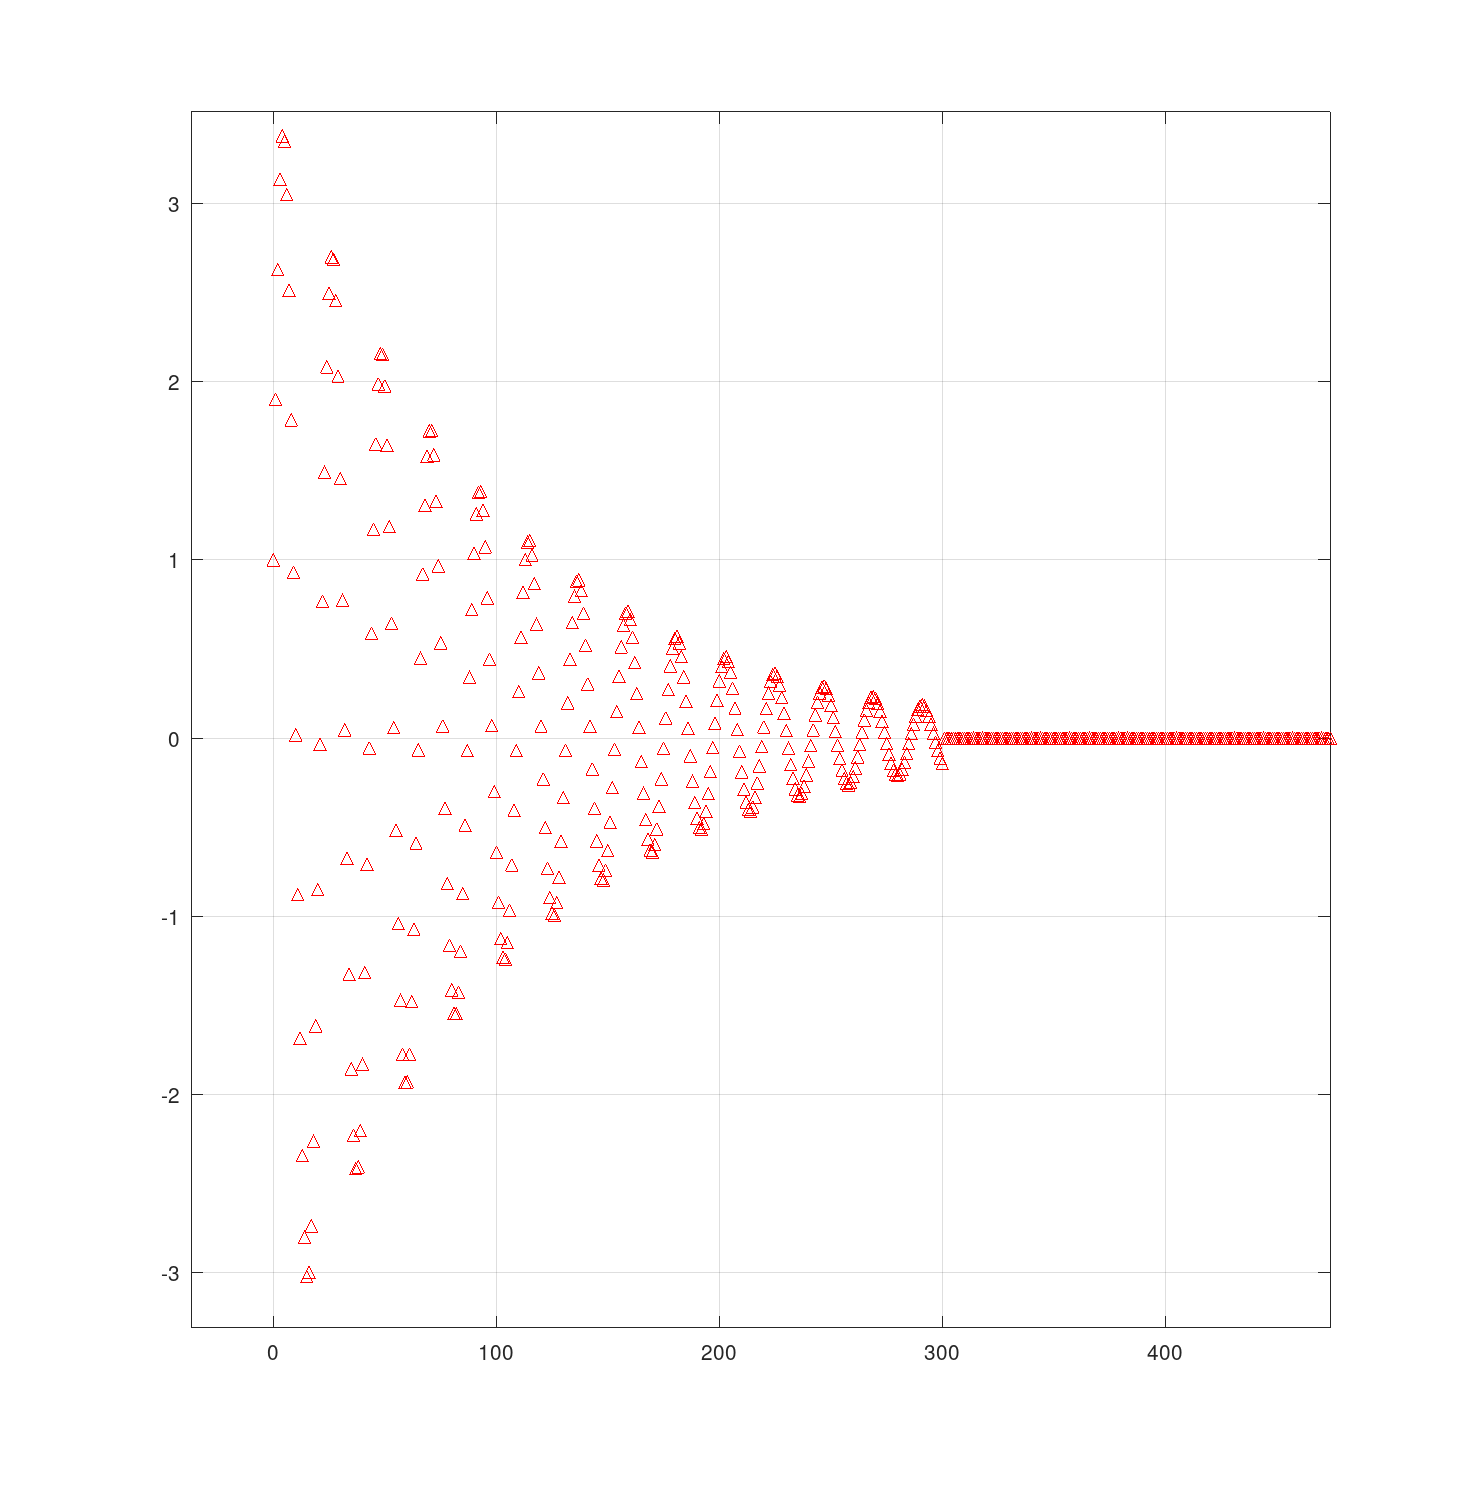
\includegraphics[width=0.52\textwidth]{../images/03-00-hfir+.png}
      \caption{Respuesta al impulso TIIR de $H_{FIR}^{+}$ según la Ec. \ref{eq:03-00-hfir+}}
      \label{fig:03-00-hfir+}
    \end{figure}

    En la Fig. \ref{fig:03-00-hfir+} se puede observar la respuesta al impulso de $H_{FIR}^{+}(z)$, donde se puede notar que efectivamente, en el paso $n=301$, la cola de la respuesta se ha subtraído.

    A continuación, se forma el sistema reverso conjugado $H_{FIR}^{-}(z)$ como se describe en la Ec. \ref{eq:47}, y se llega a

    \begin{align}
      H_{FIR}^{-}(z) =& \frac{-z \: B^{\prime -}(z) + z^{-N} \: B^{-}(z)}{A^{-}(z)} \nonumber \\
      =& \frac{-0.13977 \: z^{2} + 0.162126 \: z - z^{-N}}{0.98 \: z^{2} - 1.9 \: z +1} \nonumber \\
      =& \frac{-0.142622 \: z^{2} + 0.165435 \: z - 1.0220408 \: z^{-N}}{z^{2} - 1.938776 \: z + 1.020408}
    \end{align}

    Por lo que se pueden definir los coeficientes de $H_{FIR}^{-}(z)$ como

    \begin{itemize}
      \item $c = 0.142622$
      \item $d = 0.165435$
      \item $e = 1.020408$
      \item $u = 1.938776$
      \item $v = 1.020408$
    \end{itemize}

    Luego, se reescriben los polinomios de $H_{FIR}^{-}(z)$ de forma que sea posible computarla con GNU Octave, al igual que se realizó para $H_{FIR}^{+}(z)$

    \begin{align}
      H_{FIR}^{-}(z) =& \frac{-c \: z^{2} + d \: z - \nicefrac{e}{z^{N}}}{z^{2} - u \: z + v} \nonumber \\
      =& \frac{-c \: z^{N+2} + d \: z^{N+1} - e}{z^{N} \: \left( z^{2} - u \: z + v \right)} \nonumber \\
      =& \frac{-c \: z^{N+2} + d \: z^{N+1} - e}{z^{N+2} - u \: z^{N+1} + v \: z^{N}}
      \label{eq:03-00-hfir-}
    \end{align}

    Y se realiza entonces con la misma el algoritmo en GNU Octave como se muestra a continuación

    \lstinputlisting[language=Octave]{../code/tiir_hfir2.m}

    \begin{figure}
      \centering
      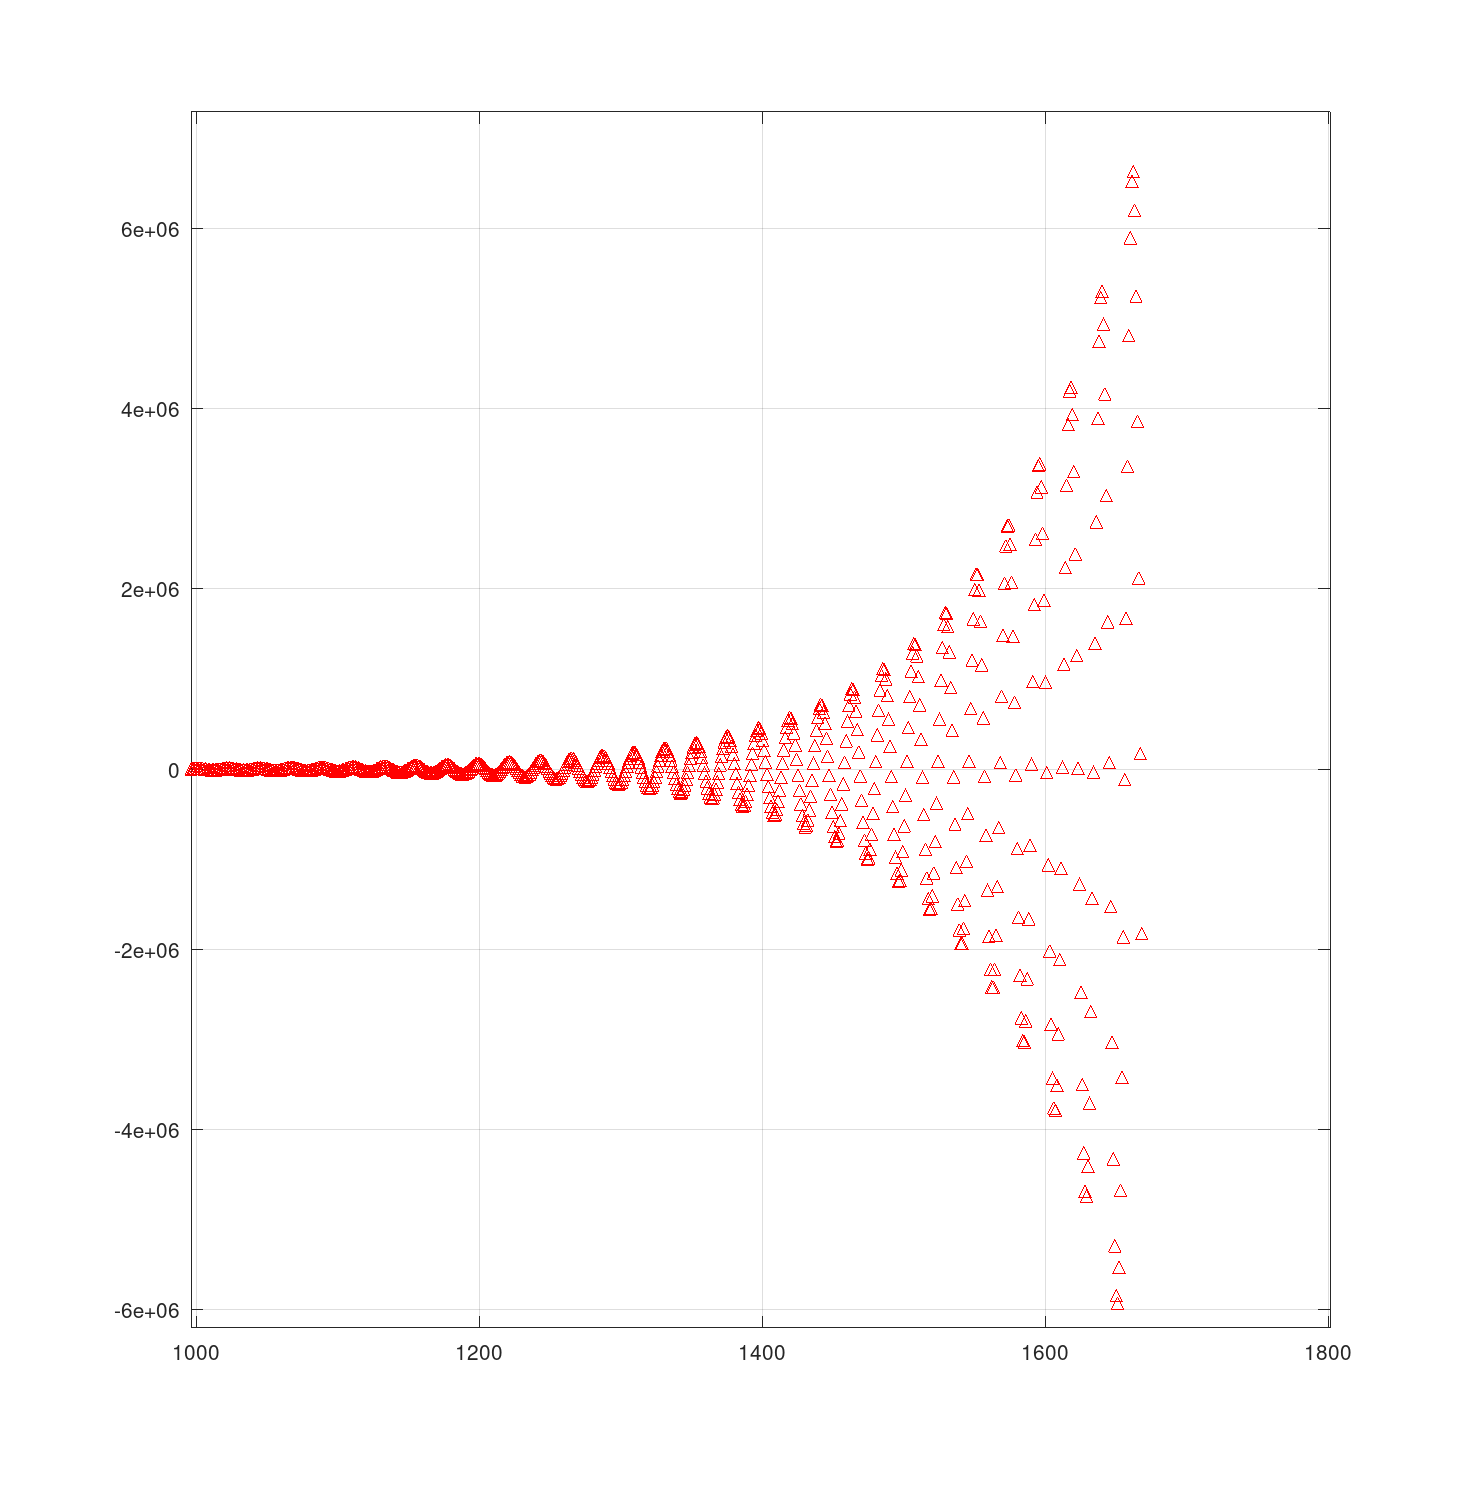
\includegraphics[width=0.5\textwidth]{../images/tiir_hfir2.png}
      \caption{Respuesta al impulso TIIR de $H_{FIR}^{-} según la Ec. \ref{eq:03-00-hfir-}$}
      \label{fig:tiir_hfir2}
    \end{figure}

    Entonces, como se puede observar en la Fig. \ref{fig:tiir_hfir2}, el sistema posee modos ocultos inestables. Se nota que, al igual que $H_{FIR}^{+}(z)$, la cola se cancela, pero sin embargo aquí el ruido de cuantización es tan grande que eventualmente abruma a la señal.

%%% Local Variables:
%%% mode: latex
%%% TeX-master: "../main"
%%% End:
